\documentclass[12pt,english]{article}
\usepackage[utf8]{inputenc}
\usepackage{tgpagella} % Palatino text only
\usepackage{mathpazo}  % Palatino math & text
% \usepackage[left=1.5in,right=1.5in,top=1.5in,bottom=1.5in]{geometry}
\usepackage[margin=1.5in]{geometry}
% \linespread{1.5}
% \usepackage[super,comma,sort]{natbib}
\usepackage[round,sort&compress]{natbib}
\usepackage{url} % [hyphens]
\usepackage[hyperpageref]{backref} % back references biblio. Needs latexmk at compilation.
\usepackage[pagebackref]{hyperref}
% \usepackage{multibib} % incompatible with backref
\hypersetup{
  colorlinks=true, % breaklinks=true,
  urlcolor=purple,    % color of external links
  linkcolor=blue,  % color of toc, list of figs etc.
  citecolor=violet,   % color of links to bibliography
}
\usepackage{bm}
\usepackage{indentfirst}
\usepackage{tocbibind}
\setcitestyle{aysep={}} 
\usepackage{amsmath}
\usepackage{amssymb}
\usepackage{eurosym}
\usepackage{amsfonts}
\usepackage{enumerate}
\usepackage{babel}
\usepackage{caption}
\usepackage{supertabular}
\usepackage{tabularx}
\usepackage{float}
\usepackage{dsfont}
\usepackage{fancyvrb}
\usepackage{verbatim}
\usepackage{enumitem}
\usepackage{setspace}
\usepackage{comment}
\usepackage{subcaption}
\usepackage{graphicx}
\usepackage{tikz}
\usepackage{gensymb}
\usepackage{textcomp}

\usepackage{tabulary}
\usepackage{tabularx}
\usepackage{booktabs}
\usepackage{fullpage}
\usepackage{morefloats}
\usepackage{makecell}
\usepackage{lscape}
\usepackage{pdflscape}
\usepackage{longtable}
\usepackage{rotating}
\usepackage{fancyhdr}
\usepackage{tocloft}
\usepackage{titletoc}
\usepackage{titlesec} % To change size of Bibliography heading
\usepackage[export]{adjustbox}
\usepackage[anythingbreaks]{breakurl} % for links
\usepackage{multicol}
\newsavebox\ltmcbox % For net gain table over two columns
%\usepackage[nomarkers,figuresonly]{endfloat} % Figures at the end
%\usepackage[section,below]{placeins} % Floats placed in the section they appear in.
\renewcommand{\floatpagefraction}{.9}

\title{Global Solidarity Advocates -- Position Paper
} 

\author{Adrien Fabre\footnote{CNRS, CIRED. E-mail: adrien.fabre@cnrs.fr (corresponding author).}} 

\date{\today{} -- \href{https://github.com/bixiou/global_tax_attitudes/raw/main/paper/position_paper.pdf}{Link to most recent version}} 

\begin{document}

\maketitle
\tikz [remember picture, overlay] %
\node [shift={(5.5cm,-1.5cm)}] at (current page.north west) % north west
[anchor=north west] % north west
{\href{http://global-redistribution-advocates.org}{
\includegraphics[height=1.3cm]{../figures/policies/logo_full_white_bg}}};

\vspace{-1cm}
\section{We need global redistribution}

%Addressing global poverty, inequalities and climate change are at the heart of the universally agreed Sustainable Development Goals (SDG). Yet, we are about to miss the SDGs as low-income countries do not have enough domestic resources to alleviate extreme poverty. 
To meet the first Sustainable Development Goal and end extreme poverty by 2030, we need international transfers. % TODO: citation
The nominal GDP per capita is \href{https://data.worldbank.org/indicator/NY.GDP.PCAP.CD?end=2021&locations=EU-ZG-XD-XM-1W-IN-US-CD-BI-LU-CN&start=2021&view=bar}{62 times larger} in high-income countries (home to 1.2 billion people) than in low-income countries (700 million). In other words, a transfer of just 1\% of high-income countries' GDP would mechanically double low-income countries' national income. A transfer of this magnitude can be financed by a modest tax on wealth above \$5 million, leaving unaffected 99.9\% of people. 

Global Redistribution Advocates call on world leaders to implement global policies redistributing at least \$1 trillion (i.e. 1\% of global income) from higher income countries to lower income countries. %Our association advocates for policies supported by strong majorities of the population in each country. Actually, 
Indeed, ``Present economic differences between rich and poor countries are too large'', as agree 78\% of people in 29 countries \citep{issp_international_2019}. %Global Redistribution Advocates is not just an association: 
In fact, we are all global redistribution advocates. % Only 5\% disagree

% Likewise, the Sustainable Development Goals set different targets for 2030, the first one being to eradicate extreme poverty defined as living on less than \$1.90 a day (in 2011 PPP). We are not on track to achieve this target, as 8\% of the world population still live in extreme poverty \citep{un_sustainable_2022}. 

% Extreme poverty is parallel to global inequality, as the GDP per capita (in 2021, in purchasing power parity) is 26 times larger in high-income countries (home to 1.2 billion people) than in low-income countries (700 million), 59 times larger in the U.S. than in the DRC, and 172 times larger in Luxembourg than in Burundi. Indeed, in each of 29 countries, \citet{issp_international_2019} uncover near consensus that ``Present economic differences between rich and poor countries are too large'' (overall, 78\% agree and 5\% disagree). A global 2\% tax on individual wealth in excess of \$5 million would collect \$816 billion every year, leaving unaffected 99.9\% of people.\footnote{Figures come from \citet{chancel_world_2022}, the \href{https://wid.world/world-wealth-tax-simulator/}{WID wealth tax simulator}, and the World Bank.} If 35\% of these potential revenues were allocated to low-income countries, their national income would increase by 50\%.

% Addressing global poverty, inequalities and climate change are at the heart of the universally agreed Sustainable Development Goals (SDG). % 12 out of  17
% It has been pointed out that low-income countries generally do not have enough domestic resources to eliminate the poverty gap in the short run.\cite{bolch_arithmetics_2022} % In other words, it would hardly be possible to achieve the first SDG an↑d end extreme poverty by 2030 without international transfers. => Careful, Bolch use a poverty line above the SDG one.

\begin{figure}[h!]
  \caption{Selected GDP per capita in PPP relative to the World's (2021, World Bank).}\label{fig:GDPpc}
  \makebox[\textwidth][c]{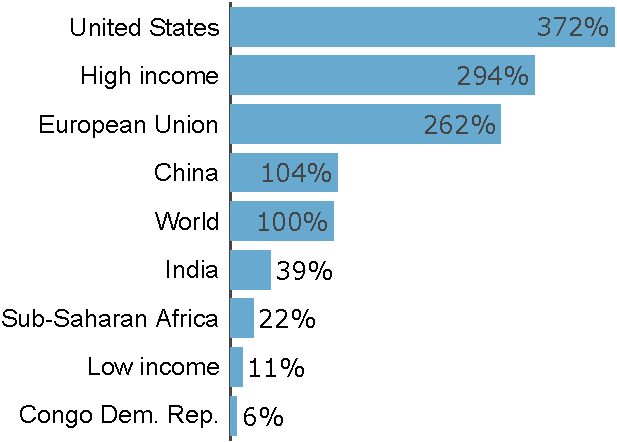
\includegraphics[width=.56\textwidth]{../figures/policies/GDP_pc_PPP_few.pdf}} % https://data.worldbank.org/indicator/NY.GDP.PCAP.PP.CD?contextual=default&end=2021&locations=EU-ZG-XD-XM-1W-IN-US-CD-BI-LU-CN&start=2021&view=bar
\end{figure}


\section{Our three policies}

Our association is structured in autonomous campaigns, one per policy. For each campaign, we write a policy brief, deploy a petition, and reach out to politicians. Our goal is that political parties throughout the world include our policies in their platform, and implement them when in power. We advocate three popular policies:
\begin{enumerate}
  \item A \href{https://github.com/bixiou/global_tax_attitudes/raw/main/paper/policy_brief_tax.pdf}{Global Wealth Tax} to finance low-income countries. Each country would tax individual wealth that is above \$5 million.\footnote{Our basic tax schedule consists of a 2\% tax on wealth above \$5 million, 4\% above \$100 million, and 6\% above \$1 billion.} 
  Half of the revenues would be pooled to finance infrastructure and public services in lower income countries. 
  \item A \href{https://github.com/bixiou/global_tax_attitudes/raw/main/paper/policy_brief_GCP.pdf}{Global Climate Plan} (GCP) to stop global warming and eradicate exteme poverty. The GCP would establish a cap on global CO$_\text{2}$ emissions, with a yearly quota that decreases in line with the climate target of the Paris agreement. Polluting firms would be required to buy emissions permits to cover their emissions. The revenues from the auction of emissions permits would finance a global basic income of about \$50 per month to each human adult. The GCP would thus lift out of extreme poverty the 700 million people who earn less than \$2 a day. The redistribution operated by the GCP would greatly benefit Africa and South Asia, and would be neutral to China. The system would also be open to subnational States like California. 
  \item A Global Assembly on Climate Change. The Global Assembly on Climate Change would be responsible for drafting international treaties against climate change. Each adult in the world would have one vote. To ensure the principle of ``one person = one vote'', the members of the assembly would be elected by proportional representation on global lists, in a single constituency.
\end{enumerate}

\begin{figure}[h!]
  \caption{Support for our three policies (in percent), from \citet{fabre_international_2023}.}\label{fig:GDPpc}
  \makebox[\textwidth][c]{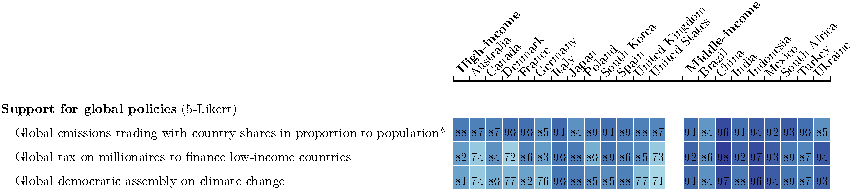
\includegraphics[width=1.2\textwidth]{../figures/OECD/Heatplot_global_tax_attitudes_3_share.pdf}} 
\end{figure}


On top of these three policies, we run a ``meta'' campaign: that such policies be discussed in international negotiations, in the UN, the COP, and the G20. 
We may campaign on more policies, as long as they are supported by strong majorities of the population in each country. 
% 2. Three policies
% Compute transfer from HIC to LIC by GCS and by millionaire tax, hoping it's 1% of global GDP.

\section{Complementarity between policies}

Our policies entail large transfers to lower income countries: 0.65\% of the global GDP with the global wealth tax and 0.9\% with the GCP (at its peak). 

These large and predictable flows of income for people and governments in lower-income countries would help lower interest rates in these countries, and spur a tide of investments. 
Our policies should be viewed as complement, not substitute, to other development and climate policies. For instance, we should not rely solely on the carbon price incentive to decarbonize. Various climate policies can complement the GCP at the national level. At the global level, financial actions are needed to de-risk low carbon projects (especially in low-income countries) and unleash green investments (\href{https://www.foreign.gov.bb/the-2022-barbados-agenda/}{Bridgetown Initiative}, \citealp{hourcade_accelerating_2021}). 

Our policies also complement each other. The Global Assembly on Climate Change could provide the ideal arena to draft the GCP and its specifics (such as the carbon budget). If negative net emissions are needed in the second half of the century, the Global Wealth Tax could provide funding for carbon removal. Besides, participating in the global wealth tax could be a condition to benefit from receiving the basic income from the GCP, to encourage lower income countries to implement the wealth tax. Similarly, the opt out provision that allows middle-income countries not to lose from the GCP could be granted only to countries that participate in the global wealth tax.

% en vrac:
% On calcule la taxe sur la fortune de sorte que ça compense le gain qu'ils obtiennent les recettes en fonction de leurs émissions territoriales plutôt que de leur empreinte. =$>$ calculer le montant nécessaire -$>$ Environ .2\% du PIB mondial pour la Chine (cf. policy\_brief\_tax avec une base de GCS=3% GWP). Si tout est reversé aux pays à bas revenus, il faut une taxe qui rapporte .2\% du PIB mondial en Chine, soit $\approx 1.2\%$ du PIB mondial en tout. Ce qui est faisable en ne s'attaquant qu'aux fortunes $>$5M et sans même les réduire (taux max de 7\%). Ça opérerait un transfert de $\approx1.2\%$ du PIB mondial, du même ordre que $\approx$133\% du GCS. À comparer au .85T\$ (surestimé, cf. calcul dans map\_GCS\_incidence.R) nécessaire pour résorber le poverty gap à 3.65\$ (il est de 4T pour le pg à 6.85\$/day) % TODO! faire ces calculs dans le position paper (ou en off)

\section{This is just a first step}

Our policies may seem utopian, but they really are the minimum we should do, to start addressing global inequalities. In line with the SDGs, our overarching goal should be to provide a decent life to all, sustainably. In the long run, we need to think ``Beyond the Welfare State'' and build a Welfare World \citep{myrdal_beyond_1960}. \citet{kopczuk_limitations_2005} compute that an optimal tax system at the global level would provide a basic income of \$250 per month, and reduce the world's Gini inequality index from 0.695 to 0.25. By comparison, implementing optimal taxes at the national level would only bring it down to 0.69. In other words, inequalities cannot be tackled at the national level. 

{\footnotesize
\begingroup
\setstretch{.5}
\titleformat*{\section}{\fontsize{11pt}{14pt}\bfseries\selectfont}
\renewcommand{\url}[1]{\href{#1}{Link}} % NCCcomment
\bibliographystyle{plainnaturl_clean} % NCCcomment
\bibliography{global_tax_attitudes}
\endgroup

}
\end{document}